
%%%%%%%%%%%%%%%%%%%%%%%%%%%%%%%%%%%%%%%%%%%%%%%%%%%%%
%
%
%  	PROBABILITY MODELS - 
%
%
%%%%%%%%%%%%%%%%%%%%%%%%%%%%%%%%%%%%%%%%%%%%%%%%%%%%%

\begin{slide}
\question

\begin{slidesonly}
	\vspace{3cm}
\end{slidesonly}

\begin{center}
\Huge 
\textcolor{LimeGreen}{Probability Models}
\end{center}

	
\end{slide}



\begin{slide}
\question

\SavedDefinitionRender{IntroProbability}

\SavedDefinitionRender{ConditionalProb}

\end{slide}

\begin{slide}

\SavedDefinitionRender{hazard}

\begin{parts}
	\item Show that $\frac{d\tilde{F}_T}{dt} = - f_T$. 
	\item Find an ODE that relates $\tilde{F}_T$ and $h(t)$ and use it to show that
	\[ \tilde{F}_T(t) = e^{-\int_{-\infty}^t h_T(\tau) ~d\tau} \]

	\item Show that the mean satisfies 
	\[\displaystyle 
		\mu_T = \int_{-\infty}^\infty \tilde{F}_T(t) ~dt.
	\]
\end{parts}
	
\end{slide}


\begin{slide}
\question \label{exponential}

\SavedDefinitionRender{Exponential}

Let us study the \textbf{exponential random variable}: 
\[T \sim {\rm Exp}(\gamma).\]

\begin{parts}
	\item Find an expression for its cdf $F_T(t)$.
	\item Find an expression for its ccdf $\tilde{F}_T(t)$.
	\item Find an expression for its hazard function $h_T(t)$.
	\item What is its mean $\mu_T$?
\end{parts}

\begin{slidesonly}
\vspace{3cm}	
\end{slidesonly}

The hazard function is a constant, so knowing that the random variable is yet to occur, doesn't us give any information.

\SavedDefinitionRender{memoryless}


\begin{parts}
\setcounter{partsitem}{4}
	\item Show that the Exponential is memoryless.
\end{parts}
	
\end{slide}


\begin{solution}
\begin{slide}
\begin{parts}

	\item $\displaystyle F_T(t) 
	 		= \int_{-\infty}^t f_T(\tau)~d\tau
	 		= \int_0^t \gamma e^{-\gamma \tau} ~d\tau
%	 		= - e^{-\gamma \tau} \big|_0^t 
	 		= 1-e^{-\gamma t}$
	 
	 \item $\tilde{F}_T(t) = 1 - F_T(t) = e^{-\gamma t}$.

	 \item $\displaystyle h_T(t) = \frac{f_T(t)}{\tilde{F}_T(t)} = \gamma$.

	 \item $\displaystyle \mu_T 
	 		= \int_{0}^\infty \tau f_T(\tau) ~d\tau
	 		= \int_0^\infty \tilde{F}_T(\tau) ~d\tau 
	 		= -\frac{1}{\gamma} e^{-\gamma \tau} \big|_0^\infty
	 		= \frac{1}{\gamma}$
	 	
	 \item 
	 $\displaystyle \Pr(T>t+s|T>t) = \frac{\Pr(T>t+s)}{\Pr(T>t)} = \frac{e^{-\gamma (t+s)}}{e^{-\gamma t}} = e^{-\gamma s} = \Pr(T>s)$.
	 
	

	
\end{parts}


	
\end{slide}

\end{solution}
	




\begin{slide}
\question

Backblaze is a cloud storage company that uses thousands of hard drives\footnote{They publish data on their hard drives \url{https://www.backblaze.com/b2/hard-drive-test-data.html}.}.\\

The failure rate for a hard drive, also known as hazard rate, is composed of three terms:
\begin{center}
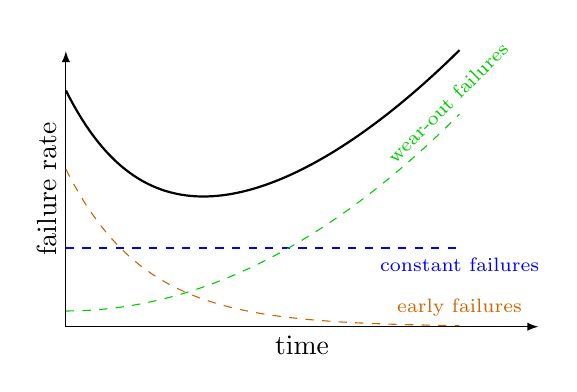
\begin{tikzpicture}
	\draw[latex-latex] (6,0) --node[below] {time} (0,0) --node[above,rotate=90] {failure rate} (0,3.5);
	\draw[dashed,blue] (0,1) -- (5,1) node[below] {\scriptsize constant failures};
   \draw[dashed,orange!80!black,variable=\x,samples=100,domain=0:5] plot({\x},{2*exp(-\x)}) node[above] {\scriptsize early failures}; 
   \draw[dashed,green!80!black,variable=\x,samples=100,domain=0:5] plot({\x},{0.2+\x*\x/10}) node[above,rotate=45] {\scriptsize wear-out failures}; 
   \draw[thick,variable=\x,samples=100,domain=0:5] plot({\x},{1+\x*\x/10+2*exp(-\x)}); 
\end{tikzpicture}
\end{center}

When we add the three terms, we get a \textit{bathtub} curve. \\

Should Backblaze always use the hard drives with the longest mean time between failures (MTBF)?

\begin{parts}
\item Suppose that there are $N$ hard drive types, each with a known fixed cost $c_n$, a known profit $p_n$ per unit time that hard drive is operational, and a random lifetime $T_n$ with a known distribution. Backblaze has limited storage, so they can only have $M$ hard drives. If they use $x_n$ drives of type $n$, what is their profit function?

%$$
%P = \sum_{n=1}^N \left[p_n \sum_{m=1}^{x_n} T_n(m)  - x_n c_n \right]
%$$

\item What is their expected profit?
%$$
%\sum_{n=1}^N \left[x_n p_n \mu_{T_n}  - x_n c_n \right]
%$$

\item If they choose to maximize the expected profit, what is the solution?
\end{parts}

	
\end{slide}


\begin{slide}

This means that they will \textit{put all their eggs in one basket}!

This is a risky strategy. Especially if hard drives with long-lives have a large variance in those lives.

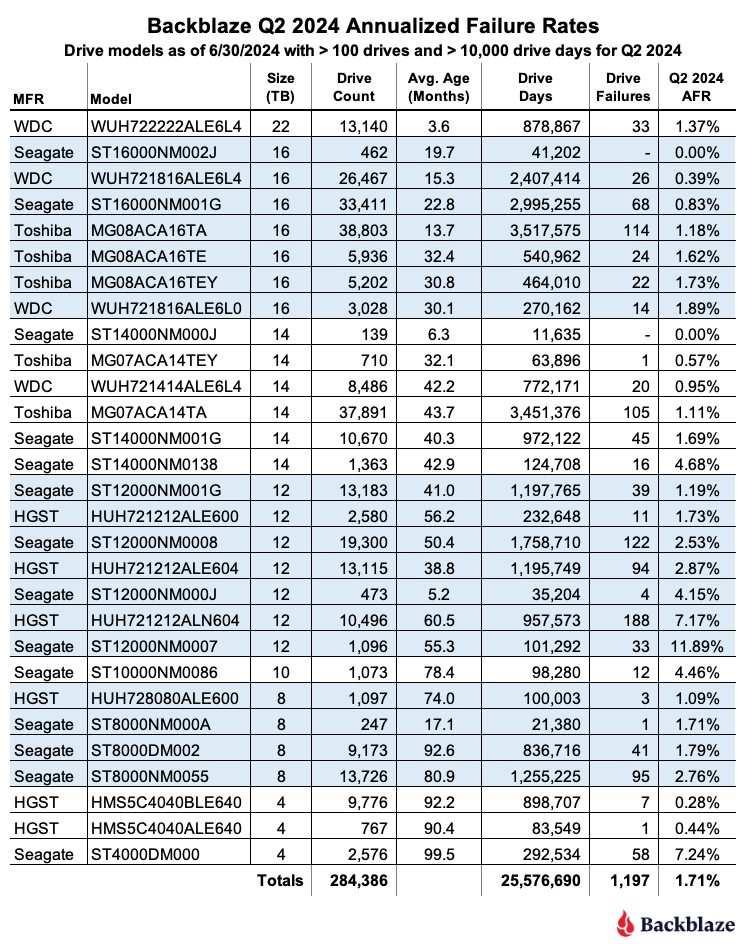
\includegraphics[width=150pt]{images/backblaze-hdd.png}

To account for this, we can add a constraint that the variance of the profit $\sigma_P^2$ not be too large.
This will result in a more diverse selection of hard drives.
Unfortunately, for most hard drive lifetime distributions, this constraint is non-linear in the decision variables. 

	
\end{slide}






\begin{slide}
\question \label{ex-poisson}

\SavedDefinitionRender{Poisson}

Start with $N(0) = 0$ and define $p_n(t) = \Pr\big( N(t)=n \big)$, the probability that $n$ events have occurred up to time $t$.


\begin{slidesonly}
	\bigskip
\end{slidesonly}

\begin{parts}
	\item What is $p_n(0)$?
	\item Take $n=0$. Explain in words why $p_0(t) = \tilde{F}_T(t)$.

	\item A different approach:
	\[ 
		\underbrace{\frac{d p_0}{dt}(t)}_{\substack{\text{change in prob}\\\text{that $N(t)=0$}}}
		 = +\underbrace{0}_{\text{can never increase}}
		 -\underbrace{p_{0}(t) h_T(t)}_{\substack{\text{decreases if $N$ was $0$}\\\text{and an event occurs}}}
	\]

	Solve this differential equation to find $p_0(t)$.

	\item For $n>0$, we can find an ODE in a similar way. The change in probability that $N(t)=n$:
	\begin{enumerate}
		\item decreases if ...
		\item increases if ...
	\end{enumerate}
	
	\item Obtain an ODE and show that $p_n(t) = \frac{(\gamma t)^n}{n!} e^{-\gamma t}$ is a solution.
	
	\item Show that it is normalized, i.e. $\displaystyle\sum_{n=0}^\infty p_n(t) = 1$.

	\item Calculate its mean $\displaystyle\sum_{n=0}^\infty n p_n(t)$.
	
	
\end{parts}

	
\end{slide}


\begin{solution}
	

\begin{slide}
\begin{parts}
	\item $p_n(0) = \delta_{n,0}$
	\item It is the probability that no events have occurred until time $t$, which is the complement of the probability of an event happening between time $0$ and $t$, so $p_0(t) = 1 - F_T(t) = \tilde{F}_T(t) = e^{-\gamma t}$.

	\item The ODE is $\frac{d p_0}{dt} = -\gamma p_0$, so the solution is $p_0(t) = e^{-\gamma t}$.

	\item 
	\begin{enumerate}
		\item increases if $N$ was $n-1$ and an event occurs imminently
		\item decreases if $N$ was $n$ and an event occurs imminently
	\end{enumerate}
	
	\item 	
	\[ 
		\underbrace{\frac{d p_n}{dt}(t)}_{\substack{\text{change in prob}\\\text{that $N(t)=n$}}}
		 = +\underbrace{p_{n-1}(t) h_T(t)}_{\substack{\text{increases if $N$ was $n-1$}\\\text{and an event occurs}}}
		 -\underbrace{p_{n}(t) h_T(t)}_{\substack{\text{decreases if $N$ was $n$}\\\text{and an event occurs}}}
	\]
	This gives 
	\[ 
		\frac{dp_n}{dt}(t) = \gamma p_{n-1}(t) - \gamma p_n(t)
	\]
	
	\item The series 
	\[ \sum_{n} \frac{(\gamma t)^n}{n!}  \]
	is the Taylor series for $e^{\gamma t}$.
	
	\item Consider $g_n(t) = \frac{(\gamma t)^n}{n!}$. Then
%	\[
%	g_n'(t) = n \frac{(\gamma t)^{n-1}}{n!}
%	\]
%	and
	\[t g_n'(t) = n g_n(t)\]
	So
	\[ \sum_n n \frac{(\gamma t)^n}{n!} 
		= t \left( \sum_n \frac{(\gamma t)^n}{n!}\right)'
		= t \left( e^{\gamma t} \right)'
		= t \gamma e^{\gamma t} \]
	Thus the mean is $E(N(t)) = \gamma t$, which is typically denoted by $\lambda$.

\end{parts}
	
\end{slide}
\end{solution}


\begin{slide}

\SavedDefinitionRender{Poisson2}
	
\end{slide}



\begin{slide}
\question
\begin{problem}[Aquarium Problem\footnote{based on a problem from Meerschaert's `Mathematical Modeling'.}]

A pet store sells large aquariums. They sell approximately \textbf{one aquarium per week} (call this the parameter $\lambda$).

Not wanting to maintain too much stock (the aquariums are large and fragile), the store orders 3 aquariums at the end of the week if they are completely out of stock.

How missed sales result from this policy?
\end{problem}

Let
\begin{itemize}
	\item $X_n = $ number of aquariums in stock at the beginning of week $n$
	\item $D_n=$ number of aquariums demanded in week $n$
\end{itemize}
Any available aquariums that are demanded are purchased and assume that when the store orders aquariums, they arrive right away.


\begin{parts}
	\item Why is $X_n$ random?
	\item Assume that $D_n$ is Poisson distributed. Why is this reasonable?
	\item Then what is $\Pr (D_n = k)$?
	\item There are only 3 states of $D_n$: 1, 2, 3. 
	
	The following diagram shows the possible changes in stock from one week to the next.
	
	Complete the following diagram with the probability of transitioning from one state to another for all the arrows except the ones marked with $\star$.
	
	\begin{center}
	\begin{tikzpicture}[font=\sffamily,scale=0.4]
	 
        % Setup the style for the states
        \tikzset{node style/.style={state, 
                                    minimum width=1cm,
                                    line width=0.3mm,
                                    fill=gray!20!white}}
 
        % Draw the states
        \node[node style] at (0, 0)     (x1)    {$X_n=1$};
        \node[node style] at (6, 0)     (x2)    {$X_n=2$};
        \node[node style] at (3, -5.196) (x3) 	{$X_n=3$};
 
        % Connect the states with arrows
        \draw[every loop,
              auto=right,
              line width=0.3mm,
              >=latex,
              draw=black,
              fill=black]
            (x1) edge[loop above]             node {} (x1)
            (x2) edge[loop above]             node {} (x2)
            (x3) edge[loop below]             node {$\star$} (x3)            
            (x1)     edge[bend right=20]            node {} (x2)
            (x2)     edge[bend right=20]            node {} (x1)
            (x1)     edge[bend right=20]            node {$\star$} (x3)
            (x3)     edge[bend left=20]            node {} (x2)
            (x2)     edge[bend left=20, auto=left] node {$\star$} (x3)
            (x3) edge[bend right=20, auto=right] node {} (x1);
    \end{tikzpicture}
	\end{center} 

	\item For the remaining arrows, marked with $\star$, observe that if there is one aquarium in inventory and 3 clients come, then the store will only be able to sell one of them and order new aquariums, so at the beginning of next week there will be 3 aquariums. Because of this, complete the  remaining $\star$ arrows by using the complementary probability. 

\end{parts}


\end{slide}


\begin{slide}

\begin{parts}
\setcounter{partsitem}{5}
	\item Create a transition matrix $\mathcal{P}$ with
	\begin{itemize}
		\item $P_{ij} = $ probability of transitioning from state $i$ to $j$
	\end{itemize}
	
	\item Let 
	\[ 
	\vec{\pi}_n = \mat{ 	\Pr(X_n = 1) \\
					\Pr(X_n = 2) \\
					\Pr(X_n = 3) }
	\]
	Find a relation between $\vec{\pi}_{n+1}$ and $\vec{\pi}_n$.
	
	\item Use \href{https://utoronto.syzygy.ca/jupyter/user-redirect/git-pull?repo=https://github.com/bigfatbernie/IBLMathModeling&subPath=book/python/aquarium.ipynb}{\tt aquarium.ipynb} to approximate the solution for the long term states. 
		Interpret the results.

	\item The original question was about how much business is the store missing. Write the expected percentage of weeks when the store lost at least one sale as a probability.
	
	\item Calculate $W$:
	\begin{align*}
	W 	& = \lim_{n \to \infty} \Pr(D_n > X_n) \\
		& = \lim_{n \to \infty} \sum_{i=1}^3 \Pr(D_n>X_n | X_n = i) \Pr (X_n = i),
	\end{align*}
	using the limiting vector $\vec{\pi}$ found. Interpret the result.
	
	\item We can calculate the average lost sales too by considering:
	\[
	L	= \lim_{n \to \infty} \sum_{i=1}^3 (D_n - i) \Pr(D_n>X_n | X_n = i) \Pr (X_n = i).
	\]
	
	Calculate $L$, the expected number of lost aquarium sales. Interpret the results.
	
	\item What is $S(L^\star, \lambda)$?
\end{parts}

	
\end{slide}




\begin{solution}
\begin{slide}
\begin{parts}
	\item Because $D_n$ is random.  
	\item Because the arrival of customers can happen at any time, they are independent of each other, and they don't depend on $t$ (in reality they do), but because we are measuring in weeks, it's ok.
	\item $\Pr(D_n=k) = \frac{\lambda^k}{k!} e^{-\lambda}$.
	\item 
	
	\begin{center}
	\begin{tikzpicture}[font=\sffamily,scale=0.5]
	 
        % Setup the style for the states
        \tikzset{node style/.style={state, 
                                    minimum width=1cm,
                                    line width=0.3mm,
                                    draw=black,
                                    fill=gray!20!white}}
 
        % Draw the states
        \node[node style] at (0, 0)     (x1)    {\textcolor{black}{$X_n=1$}};
        \node[node style] at (6, 0)     (x2)    {\textcolor{black}{$X_n=2$}};
        \node[node style] at (3, -5.196) (x3) 	{\textcolor{black}{$X_n=3$}};
 
        % Connect the states with arrows
        \draw[every loop,
              auto=right,
              line width=0.3mm,
              >=latex,
              draw=black,
              fill=black]
            (x1) edge[loop above]             node {$e^{-\lambda}$} (x1)
            (x2) edge[loop above]             node {$e^{-\lambda}$} (x2)
            (x3) edge[loop below]             node {$1-\lambda e^{-\lambda}-\frac{\lambda^2}{2}e^{-\lambda}$} (x3)            
            (x2)     edge[bend right=20]            node {$\lambda e^{-\lambda}$} (x1)
            (x1)     edge[bend right=20]            node {$1-e^{-\lambda}$} (x3)
            (x3)     edge[bend left=20]            node {$\lambda e^{-\lambda}$} (x2)
            (x2)     edge[bend left=20, auto=left] node {$1-e^{-\lambda}-\lambda e^{-\lambda}$} (x3)
            (x3) edge[bend right=20, auto=right] node {$\frac{\lambda^2}{2}e^{-\lambda}$} (x1);
    \end{tikzpicture}
	\end{center} 
	
%\setcounter{partsitem}{5}	
%
%	\item \[ 
%			\mathcal{P} 
%				= \mat{ 	e^{-\lambda} & 0 & 1 - e^{-\lambda} \\
%						\lambda e^{-\lambda} & e^{-\lambda} & 1 - e^{-\lambda} - \lambda e^{-\lambda} \\
%						\frac{\lambda^2}{2} e^{-\lambda} & \lambda e^{-\lambda} & 1 - \lambda e^{-\lambda} - \frac{\lambda^2}{2}e^{-\lambda} }
%			\]
%
\end{parts}
	
\end{slide}

\begin{slide}
\begin{parts}
\setcounter{partsitem}{5}	

	\item \[ 
			\mathcal{P} 
				= \mat{ 	e^{-\lambda} & 0 & 1 - e^{-\lambda} \\
						\lambda e^{-\lambda} & e^{-\lambda} & 1 - e^{-\lambda} - \lambda e^{-\lambda} \\
						\frac{\lambda^2}{2} e^{-\lambda} & \lambda e^{-\lambda} & 1 - \lambda e^{-\lambda} - \frac{\lambda^2}{2}e^{-\lambda} }
			\]

	\item We have $\vec{\pi}_{n+1} = \vec{\pi}_n \mathcal{P} 
		 				\quad \Leftrightarrow \quad \vec{\pi}_{n+1} = \mathcal{P}^T \vec{\pi}_n$.
	\item The long term result is: $\vec{\pi} = \mat{0.28471134 \\0.26313999 \\0.45214867}$.


	This means that with $\lambda =1$, that is with 1 expected customer per week, the store should expect to have :
	\begin{itemize}
		\item 1 aquarium in inventory 28.5\% of the weeks
		\item 2 aquariums in inventory 26.3\% of the weeks
		\item 3 aquariums in inventory 45.2\% of the weeks
	\end{itemize}
	
	This means that about half of the time, they have a full inventory. Perhaps this is due to the fact that they ran out of aquariums and just ordered more, so they might be losing a lot of sales when they run out of stock.
	
	\item It is the probability that the demand is higher than the inventory: $\Pr(D_n > X_n)$. 
	
	\begin{slidesonly}
		\bigskip	
	\end{slidesonly}

	\item $W$ is the long term expected percentage of weeks when sales are lost:\\[-20pt]
	\begin{align*}
		W 	
			& = \lim_{n \to \infty} \sum_{i=1}^3 \Pr(D_n>X_n | X_n = i) \Pr (X_n = i) \\
			& = \lim_{n \to \infty} \sum_{i=1}^3 \Pr (X_n = i) \sum_{j=i+1}^\infty \Pr(D_n=j)\\
			& = \sum_{i=1}^3 \pi_i \sum_{j=i+1}^\infty \frac{\lambda^j}{j!} e^{-\lambda} \\
			& = e^{-\lambda} \left[ \pi_1 \sum_{j=2}^\infty \frac{\lambda^j}{j!} + \pi_2  \sum_{j=3}^\infty \frac{\lambda^j}{j!} + \pi_3  \sum_{j=4}^\infty \frac{\lambda^j}{j!} \right]
	\end{align*}
	The series in $j$ is the tail of the Taylor series for the exponential $e^{\lambda}$, so we can write it as \\[-15pt]
	\begin{align*}
	W = & e^{-\lambda}  \left[ \pi_1 ( e^\lambda - 1 - \lambda ) + \pi_2 ( e^\lambda - 1 - \lambda - {\textstyle \frac{\lambda^2}{2}}) \right.\\ 
		& \left.+ \pi_3 ( e^\lambda - 1 - \lambda - {\textstyle \frac{\lambda^2}{2}- \frac{\lambda^3}{6}}) \right]
	\end{align*}
%	\begin{align*}
%	W = &   \left[ \pi_1 ( 1 - (1 + \lambda)e^{-\lambda} ) + \pi_2 ( 1 - (1 + \lambda + {\textstyle \frac{\lambda^2}{2}})e^{-\lambda}) \right.\\ 
%		& \left.+ \pi_3 (1 - (1 + \lambda + {\textstyle \frac{\lambda^2}{2} + \frac{\lambda^3}{6}})e^{-\lambda}) \right]
%	\end{align*}


	Using \href{https://utoronto.syzygy.ca/jupyter/user-redirect/git-pull?repo=https://github.com/bigfatbernie/IBLMathModeling&subPath=book/python/aquarium-sol.ipynb}{\tt aquarium-sol.ipynb}, we get $W = 0.105$, which means that the store loses sales about 11\% of the weeks.
	
\end{parts}


\end{slide}


\begin{slide}
\begin{parts}
\setcounter{partsitem}{10}
	\item Similarly, we can calculate $L =  0.14256$, so the store should expect to lose an average of 0.14 sales per week. 
	Given that the expected number of sales is 1 per week, this is about 14\% of their business and it might be worthwhile to re-evaluate their stocking policy. 
	
	\item To calculate the sensitivity, we need the approximate formula:
	\[
	S(L,\lambda) \approx \frac{L(1+\Delta)-L(1)}{\Delta} \cdot \frac{1}{L(1)} = 1.859
	\]
	
	Which is just moderately sensitive to $\lambda$.

\end{parts}

\rule{\textwidth}{0.4pt}

I also calculated the expected number of sales (should be less than $\lambda$ since we are losing some sales):
\begin{align*}
E % & = \sum_{i=1}^3 \sum_{j=1}^\infty P(D_n=j) P(X_n=i) S_{ij}\\
	& = \sum_{i=1}^3 \sum_{j=1}^i j P(D_n=j) P(X_n=i) + \sum_{i=1}^3 \sum_{j=i+1}^\infty i P(D_n=j) P(X_n=i)\\
 & = \sum_{i=1}^3 \sum_{j=1}^i j \frac{\lambda^j}{j!} e^{-\lambda}\pi_i + \sum_{i=1}^3 \sum_{j=i+1}^\infty i \frac{\lambda^j}{j!} e^{-\lambda} \pi_i \\
 & = e^{-\lambda} \left[\sum_{i=1}^3 \pi_i \lambda \sum_{j=0}^{i-1} \frac{\lambda^j}{j!} \pi_i + \sum_{i=1}^3 i \pi_i \sum_{j=i+1}^\infty i \frac{\lambda^j}{j!} \right] \\ 
 & = 0.857 \quad \text{ for }\lambda=1.
\end{align*}
So the store only makes about 85.7\% of possible sales.

\rule{\textwidth}{0.4pt}

I ran the code for values of $\lambda \in (0,10]$ to get the plots:

\begin{center}
	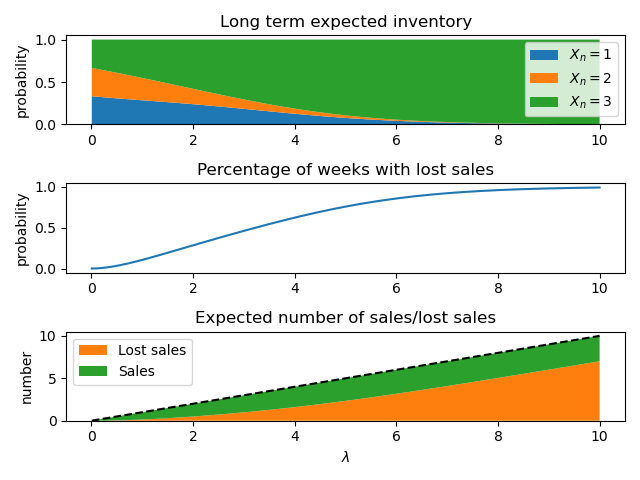
\includegraphics[width=200pt]{images/aquarium.png}
\end{center}

Observe how the number of sales converges to $3$ as $\lambda \to \infty$, which makes sense since that is the maximum inventory. The more clients that come to the store, the more likely to sell all the inventory every week.


	
\end{slide}

\end{solution}



\begin{slide}
\question

Construct a Markov chain model for the heat equation interpreting it as particles randomly bumping around and averaging their temperature when they meet.

	
\end{slide}




\begin{slide}
\begin{problem}[Stochastic Simulation]
It is very rare to be able to obtain analytic results for probabilistic models, so we will study simulating them.
\end{problem}

\SavedDefinitionRender{discrete-event}

\SavedDefinitionRender{tau-leaping}



	
\end{slide}

